\documentclass[11pt]{article}
% Кодировка и язык
\usepackage[utf8]{inputenc}           % Кодировка исходного файла (UTF-8)
\usepackage[T2A]{fontenc}             % Кодировка шрифтов для кириллицы
\usepackage[english,russian]{babel}   % Локализация: русские названия, переносы

% Поиск в PDF
\usepackage{cmap}                     

% Поля страницы
\usepackage{geometry}
\geometry{left=2cm, right=2cm, top=2cm, bottom=2cm}

% Математика
\usepackage{amsmath, amssymb, amsthm} % Базовые пакеты для математики
\usepackage{mathtools}                % Расширение amsmath (доп. символы и окружения)

% Картинки
\usepackage{graphicx}                 % Вставка картинок (\includegraphics)
\graphicspath{{pictures/}}            % Путь к папке с картинками
\usepackage{float}                    % Позволяет использовать [H] для жёсткого позиционирования
\usepackage{wrapfig}                  % Обтекание текста вокруг картинок

% Таблицы
\usepackage{array}                    % Расширенные возможности для таблиц
\usepackage{booktabs}                 % Красивые таблицы (\toprule, \midrule, \bottomrule)
\usepackage{multirow}                 % Объединение строк в таблицах
\usepackage{tabularx}                 % Таблицы с автоматической шириной колонок
\usepackage{ragged2e}                 % Улучшенное выравнивание (используется в tabularx)

% Списки
\usepackage{enumitem}                 % Гибкая настройка списков (itemize, enumerate)

% Колонтитулы
\usepackage{fancyhdr}                 

% Гиперссылки
\usepackage{xcolor}                   % Работа с цветами
\usepackage{hyperref}                 % Гиперссылки, оглавление, перекрёстные ссылки

% Умные ссылки
\usepackage{cleveref}                 

% Типографика
\usepackage[expansion=false]{microtype}                % Улучшает переносы и межсловные расстояния

% Подписи к картинкам и таблицам
\usepackage{caption}                  % Настройка подписей (шрифт, отступы)

% Рисование схем и графиков
\usepackage{tikz}                     % Рисование схем, графиков, диаграмм
\usepackage{pgfplots}                 % Построение графиков функций (на основе tikz)
\pgfplotsset{compat=newest}           % Версия совместимости pgfplots

% Алгоритмы и код
\usepackage{algorithm}                % Окружения для алгоритмов
\usepackage{algorithmic}              % Синтаксис для алгоритмов
\usepackage{listings}                 % Вставка кода с подсветкой синтаксиса


% Настройка нумерации секций и подсекций
\renewcommand{\thesection}{\arabic{section}}                   
\renewcommand{\thesubsection}{\thesection.\arabic{subsection}} 


% Настройка списков: убираем лишние отступы слева
\setlist[itemize]{leftmargin=*}
\setlist[enumerate]{leftmargin=*}


% Определение окружений для теорем, лемм, определений и т.д.
% Нумерация привязана к номеру секции
\newtheorem{theorem}{Теорема}[section]
\newtheorem{definition}{Определение}[section]
\newtheorem{remark}{Замечание}[section]
\newtheorem{lemma}{Лемма}[section]
\newtheorem{example}{Пример}[section]
\newtheorem{consequence}{Следствие}[section]
\newtheorem{algorithmm}{Алгоритм}
\newtheorem{question}{Вопрос}[section]
\newtheorem{answer}{Ответ}[section]
\newtheorem{statement}{Утверждение}[section]


% Определение цветов
\definecolor{pblue}{rgb}{0.13,0.13,1}    
\definecolor{pgreen}{rgb}{0,0.5,0}       
\definecolor{pred}{rgb}{0.9,0,0}         
\definecolor{pgrey}{rgb}{0.46,0.45,0.48}

\DeclareMathOperator{\SAT}{SAT}
\DeclareMathOperator{\tSAT}{3-SAT}
\DeclareMathOperator{\MtSAT}{MAX-3-SAT}
\DeclareMathOperator{\BPP}{BPP}
\DeclareMathOperator{\PP}{PP}
\DeclareMathOperator{\RP}{RP}
\DeclareMathOperator{\coRP}{coRP}
\DeclareMathOperator{\ZPP}{ZPP}
\DeclareMathOperator{\Poly}{P}
\DeclareMathOperator{\NotDet}{N}
\DeclareMathOperator{\NP}{NP}
\DeclareMathOperator{\poly}{poly}

\newcommand{\lectureNumber}{8}
\newcommand{\lectureTitle}{Вероятностные ДМТ. Вероятностные сложностные классы. Дерандомизация}
\newcommand{\courseName}{Формальные языки и сложность вычислений}
\newcommand{\semester}{3 семестр, 2026/2027 уч. год}

\pagestyle{fancy}
\fancyhf{}
\fancyhead[L]{Чил аут окончен, ребятки, свага накоплена}
\fancyhead[R]{\thepage}
\setlength{\headheight}{15pt}

\hypersetup{
    colorlinks=true,
    linkcolor=blue!70!black,
    citecolor=blue!70!black,
    filecolor=blue!70!black,
    urlcolor=blue!70!black,
}

\begin{document}


\begin{titlepage}
    \centering
    
    {\large Московский физико-технический институт \par}
    {\large Высшая школа программной инженерии \par}
    \vspace{2cm}

    {\Large \textbf{\courseName} \par}
    {\large \semester \par}
    
    \vspace*{\fill}

    {\Huge \textbf{Лекция \lectureNumber} \par}
    {\Huge \textbf{\lectureTitle} \par}
    
    \vspace*{\fill}
    
    {\large Лектор: Зухба Анастасия Викторовна \par}
    {\large Автор: \href{https://t.me/ceagest}{Юра} \par}

\end{titlepage}

\pagenumbering{arabic}

\section{Вероятностные вычисления}

\begin{definition}
    \textbf{Вероятностная МТ} --- ДМТ $M$ с двумя аргументами:
    \begin{itemize}
        \item $x$ (собственно аргумент),
        \item $r$ (случайные биты).
    \end{itemize}
\end{definition} \leavevmode
\\
Может показаться странным, что машина $M(x, r)$ одновременно детерминированная и вероятностная. Давайте распутываться.
Детерминированная она потому, что, имея $x$ и $r$, к примеру, на двух разных лентах, дальше все переходы определены однозначно. Вся вероятностность, на самом деле, зашита в $r$. На $x$ мы влияем сами --- его подаем на вход машине. На $r$ же мы влиять не в силах --- можно считать, что при запуске машины $M$ с указанным нами иксом, эти случайные биты уже материализовались на соответствующей ленте, и дальше мы как то с ними работаем.
\begin{definition}
    \textbf{Результат работы} $\,M(x, r)$ --- вероятностное распределение, индуцированное конкретным выбором $x$ и равномерным распределением на всех значениях $r$.
\end{definition}

\begin{definition}
    \textbf{Время работы} машины $M$ на данном $x$ --- максимальное время работы $M(x, r)$ для всех $r$ указанной длины.
\end{definition}

\subsection{Полиномиальная вероятностная ДМТ}

\begin{definition}
    ДМТ $M$ называется \textbf{полиномиальной вероятностной МТ}, если существует полином $p$ такой, что на входе $x \in \{0, 1\}^{\ast}$ и любом $r \in \{0, 1\}^{p(\left\lvert x \right\rvert)}$ машина $M$ останавливается не более, чем за $p(\left\lvert x \right\rvert)$ шагов.
\end{definition} \leavevmode
\\
Мы считаем ответом машины случайную величину $M(x, U(2^{p(\left\lvert x \right\rvert)}))$, где $U(m)$ обозначает дискретное равномерное распределение на $m$ значениях. \\
Поскольку результатом работы является случайная величина, для определения различных классов необходимо оценивать вероятности ответов и ошибок при этих ответах.

\subsection{Два вида классов}

Глобально у нас есть два вида вероятностных сложностных классов:

\begin{itemize}
    \item Время работы всегда ограниченно полиномом по $x$, но машина может ошибаться (при некоторых наборах случайных битов). Представители здесь: $\BPP$, $\PP$, $\RP$, $\coRP$. Мы по большей части будем работать с этим видом.
    \item Машина не ошибается, но время работы может зависеть от случайных битов (и не всегда полиномиальное). Этот вид представляет лишь один красавец: $\ZPP$. Этот вид мы практически не затронем.
\end{itemize}

\subsection{Класс $\ZPP$}

\begin{definition}
    Классом $\ZPP$ называется множество $\mathcal{A}$ языков $L \in \mathcal{A}$, для которых существует вероятностный алгоритм $V$ такой, что $x \in L$ при всех $r$ эквивалентно $V(x, r) = 1$, а для каждого $x$ ожидаемое по $r$ время работы \textbf{полиномиально}.
\end{definition}

\subsection{Класс $\BPP$}

\begin{definition}
    Классом $\BPP$ называется класс $\mathcal{A}$ языков $L \in \mathcal{A}$, для которых существует \textbf{полиномиальный в худшем случае} вероятностный алгоритм $V$ такой, что:
    \[x \in L \implies P[V(x, r) = 1] \geq \frac{2}{3}\]
    \[x \not \in L \implies P[V(x, r) = 1] \leq \frac{1}{3}\]
\end{definition}

\begin{remark}
    На самом деле, число $\frac{1}{3}$ здесь было выбрано произвольно: если вместо него выбрать любое число $p$, строго меньше $\frac{1}{2}$, то получится тот же самый класс. Мы покажем это ниже при помощи \textbf{амплификации}.
\end{remark}

\subsection{Амплификация}

Пусть есть полиномиальная вероятностная МТ $V(x, r)$, распознающая язык $L$ с вероятностью ошибки $p < \frac{1}{2}$. Выполним $2m + 1$ запусков этой машины, ответ получим голосованием большинством, то есть результатом будет $0$, если за $2m + 1$ запусков он встретился чаще $1$, иначе $1$. \\
Пусть $x \in L$. Тогда $x$ будет отвергнуто, если нулей будет строго больше, чем единиц, то есть количество единиц $k \in \{0, \ldots, m\}$. Для каждого такого фиксированного $k$ есть $C_{2m + 1}^k$ способов расставить $k$ единиц на $2m + 1$ мест, вероятность получить единицу есть $(1 - p)$, а ноль --- $p$. Следовательно, вероятность того, что $x$ будет отвергнуто, определяется суммой:
\[\sum_{k = 0}^m C_{2m + 1}^k (1 - p)^k p^{2m + 1 - k} = ((1-p)p)^{\frac{2m + 1}{2}} \left[\sum_{k = 0}^m C_{2m + 1}^k \left(\frac{p}{1 - p}\right)^{\frac{2m + 1}{2} - k}\right]\]
Так как $p < \frac{1}{2} < 1 - p$, то $\frac{p}{1 - p} < 1$.
Кроме того, $k \leq m$, откуда показатель $\frac{2m + 1}{2} - k > 0$. Тогда:
\[((1-p)p)^{\frac{2m + 1}{2}} \left[\sum_{k = 0}^m C_{2m + 1}^k \left(\frac{p}{1 - p}\right)^{\frac{2m + 1}{2} - k}\right] \leq ((1 - p)p)^{\frac{2m + 1}{2}} \left[\sum_{k = 0}^m C_{2m + 1}^k \cdot 1\right] \leq \]
\[\leq ((1 - p)p)^{\frac{2m + 1}{2}} \left[\sum_{k = 0}^{2m + 1} C_{2m + 1}^k\right] = ((1 - p)p)^{\frac{2m + 1}{2}} \cdot 2^{2m + 1} = \left(2\sqrt{(1 - p)p}\right)^{2m + 1}\]
Так как $p < \frac{1}{2}$, то $p, (1 - p) > 0$. Следовательно, по неравенству о средних:
\[2\sqrt{(1 - p)p} < (1 - p) + p = 1 \implies \left(2\sqrt{(1 - p)p}\right)^{2m + 1} < 1\]
Причём равенство единице не достигается, так как $p \neq (1 - p)$. \\
Если $x$ было бы выбрано не из $L$, то мы бы проделали ровно те же самые действия, и получили бы ту же оценку на вероятность ошибки. \\
Пусть $\delta = 2\sqrt{(1 - p)p}$. Получается, что какое бы $p$ не было задано изначально, мы вычислим по нему $\delta < 1$, и, в силу $\delta^n \to 0, \; n \to \infty$, мы всегда найдём такое количество запусков $m$, что $\delta^{2m + 1}$ станет меньше любой наперед заданной точности. Остался лишь один ньюансик --- мы не можем делать неполиномальное число запусков, так как иначе время работы перестанет быть полиномиальным, а это нам терять совсем не хочется. Посему нам хочется понять, почему же для любой заданной точности мы сможем найти такое $m = \poly(\left\lvert x \right\rvert)$, что $\delta^{2m + 1}$ станет меньше этой точности.
Но это совсем очевидно, друзья, ведь из матана первого курса мы знаем, что при фиксированном $n > 1$ последовательность $n^k \to +\infty, \; k \to \infty$, а значит мы всегда найдем такое $k \in \mathbb{N}$, что $\delta^{n^k}$ станет меньше любой наперед заданной точности. При этом, если изначально время работы машины $V(x, r)$ оценивалось полиномом $n^l$, где $n = \left\lvert x \right\rvert$, то время работы построенного алгоритма для заданной точности будет оцениваться полиномом $n^{l + k}$.

\subsection{Класс $\BPP_{\alpha(n), \beta(n)}$}

\begin{definition}
    Пусть $\alpha(n), \beta(n) \colon \mathbb{N} \to [0, 1]$ такие, что $0 \leq \alpha(n) < \beta(n) \leq 1$ для всех $n \in \mathbb{N}$. \\
    Классом $\BPP_{\alpha(n), \beta(n)}$ назовём множество $\mathcal{A}$ таких языков $L \in \mathcal{A}$, для которых существует полиномиальный в худшем случае вероятностный алгоритм $V$ такой, что:
    \[x \in L \implies P[V(x, r) = 1] \geq \beta(\left\lvert x \right\rvert)\]
    \[x \not \in L \implies P[V(x, r) = 1] \leq \alpha(\left\lvert x \right\rvert)\]
\end{definition}

\begin{remark}
    Задавая различные $\alpha(n)$ и $\beta(n)$, можно получить многие различные классы $($даже класс $\NP$$)$.
\end{remark}

\subsection{Класс $\BPP_p$}

\begin{definition}
    Обозначим через $\BPP_p$ аналог $\BPP$, где все вероятности берутся по распределению на $r$ такому, что его биты независимы и равны нулю с вероятностью $p$, а единице с вероятностью $(1 - p)$.
\end{definition}

\begin{statement}
    \[\forall p \in (0, 1) \; \; \BPP \subset \BPP_p\]
\end{statement}

\begin{proof}
    Требуемое тривиально получается при помощи амплификации.
\end{proof}

\begin{statement}
    Если $p \in (0, 1)$ --- полиномиально вероятностно вычислимое число, то есть $i$-ый знак его двоичного разложения можно получить вероятностным алгоритмом за полиномиальное от $i$ время, то $\BPP_p = \BPP$. \\
    Для некоторых невычислимых $p$ класс $\BPP_p$ шире $\BPP$. Такие $p$ образуют всюду плотное множество на $(0, 1)$.
\end{statement}

\subsection{Вероятностные сложностные классы}

Всюду далее, если не оговорено иного, $M$ --- полиномиальная вероятностная МТ.
\paragraph{Класс $\PP$}
\[
\renewcommand{\arraystretch}{1.5}
\begin{array}{c|c|c}
\PP & M(x,r)=1 & M(x,r)=0 \\ \hline
x \in L    & > 1/2    & < 1/2    \\ \hline
x \notin L & < 1/2    & > 1/2
\end{array}
\]
На самом деле, мы можем немного отделить вероятность ошибки от $\frac{1}{2}$. Пусть время работы $M(x, r)$ ограниченно полиномом $p(\left\lvert x \right\rvert)$, а вероятность ошибки есть $p$. 
Так как $r \in \{0, 1\}^{p(\left\lvert x \right\rvert)}$, то всего есть $2^{p(\left\lvert x \right\rvert)}$ различных значений $r$. Если бы $p$ равнялось в точности $\frac{1}{2}$, то ровно для половины значений $r$ машина $M$ выдавала бы неправильный ответ. Но $p < \frac{1}{2}$, а значит машина выдаёт неправильный ответ не более, чем для $2^{p(\left\lvert x \right\rvert) - 1} - 1$ значений $r$. Следовательно,
\[p \leq \frac{2^{p(\left\lvert x \right\rvert) - 1} - 1}{2^{p(\left\lvert x \right\rvert)}} = \frac{1}{2} - \left(\frac{1}{2}\right)^{p(\left\lvert x \right\rvert)}\]
Таким образом, проблема не в том, что мы совсем не можем отделить вероятность ошибки от $\frac{1}{2}$, а в том, что величина в правой части оценки выше зависит от $\left\lvert x \right\rvert$, да ещё и экспоненциально.
\paragraph{Класс $\RP$}
\[
\renewcommand{\arraystretch}{1.5}
\begin{array}{c|c|c}
\RP & M(x,r)=1 & M(x,r)=0 \\ \hline
x \in L    & \geq 1/2    & \leq 1/2    \\ \hline
x \notin L &  0    &  1
\end{array}
\]
\paragraph{Класс $\coRP$}
\[
\renewcommand{\arraystretch}{1.5}
\begin{array}{c|c|c}
\coRP & M(x,r)=1 & M(x,r)=0 \\ \hline
x \in L    & 1    & 0    \\ \hline
x \notin L &  \leq 1/2    &  \geq 1/2
\end{array}
\]

\subsection{Дерандомизация}

У вероятностных алгоритмов есть некоторые проблемки:

\begin{itemize}
    \item Могут с некоторой вероятностью ошибаться
    \item При реализации на практике часто используют генератор псевдослучайных чисел, что может спровоцировать отклонение из поведения от теоретического.
\end{itemize}

\begin{definition}
    \textbf{Дерандомизация} --- это процесс удаления случайности (или её минимального использования).
\end{definition} \leavevmode
\\
На самом деле это звучит как то слишком абстрактно и непонятно. Давайте разберемся на примере. \\
Вспомним оптимизационную постановку задачи $\tSAT$ --- $\MtSAT$, то есть мы хотим, чтобы было выполнено как можно больше дизъюнктов. Построим алгоритм, который гарантирует выполнимость не менее $\frac{7}{8}$ всех дизъюнктов.
\begin{figure}[h]
\centering
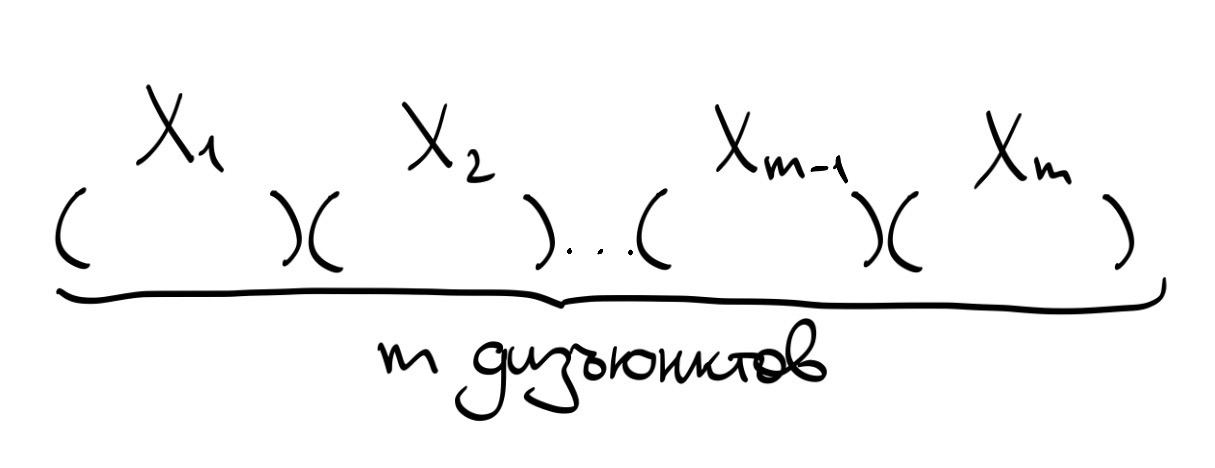
\includegraphics[width=0.6\linewidth]{дерандомизация 3-SAT.jpg}
\end{figure} \leavevmode
\\
Пусть наш вероятностный алгоритм случайно и независимо выставляет значения всех переменных в $0$ или $1$. Тогда очевидно, что вероятность того, что произвольным образом выбранный дизъюнкт обратится в истину, равна $\frac{7}{8}$. \\
Для каждого $i \in \{1, \ldots, m\}$ определим случайную величину
\begin{equation*}
    X_i = 
    \begin{cases}
        1, \text{ если дизъюнкт под номером } i \text{ выполнен} \\
        0, \text{ иначе}
    \end{cases}
\end{equation*}
Тогда $P[X_i = 1] = \frac{7}{8}$. Определим также случайную величину $X = X_1 + \ldots + X_m$. Ясно, что $X$ суть количество выполненных дизъюнктов. Тогда из линейности мат ожидания:
\[E[X] = \frac{7}{8}m\]
Теперь займёмся дерандомизацией описанного выше красавчика. \\
\underline{\textbf{Алгоритм}}: Положим изначально $x_1 = 1$. Понятно, что мы легко можем пересчитать условные мат ожидания $E[X_i \; | \; x_1 = 1]$:
\begin{equation*}
    E[X_i \; | \; x_1 = 1] = 
    \begin{cases}
        1, \text{ если дизъюнкт под номером } i \text{ содержит } x_1 \\
        \frac{3}{4}, \text{ если дизъюнкт под номером } i \text{ содержит } \overline{x}_1 \\
        \frac{7}{8}, \text{ иначе}
    \end{cases}
\end{equation*}
Тогда мы и $E[X \; | \; x_1 = 1]$ легко пересчитаем. Затем сравниваем $E[X \; | \; x_1 = 1]$ с $E[X]$. Если первое не меньше, то оставляем $x_1 = 1$, иначе полагаем $x_1 = 0$.
Из равенства
\[E[X] = \frac{1}{2} E[X \; | \; x_1 = 1] + \frac{1}{2} E[X \; | \; x_1 = 0]\]
вытекает, что мат ожидание не уменьшилось. \\
Повторяя аналогичную процедуру далее для $x_2, \ldots, x_n$, в итоге в силу неубывания мат ожидания получим не менее $\frac{7}{8}m$ выполненных дизъюнктов, что и требовалось.

\end{document}